\let\negmedspace\undefined
\let\negthickspace\undefined
\documentclass[journal]{IEEEtran}
\usepackage[a5paper, margin=10mm, onecolumn]{geometry}
%\usepackage{lmodern} % Uncomment if needed for pdflatex
\usepackage{tfrupee} % Include tfrupee package

\setlength{\headheight}{1cm} % Set the height of the header box
\setlength{\headsep}{0mm}     % Set the distance between the header box and the top of the text

\usepackage{gvv-book}
\usepackage{gvv}
\usepackage{cite}
\usepackage{amsmath,amssymb,amsfonts,amsthm}
\usepackage{algorithmic}
\usepackage{graphicx}
\usepackage{textcomp}
\usepackage{xcolor}
\usepackage{txfonts}
\usepackage{listings}
\usepackage{enumitem}
\usepackage{mathtools}
\usepackage{gensymb}
\usepackage{comment}
\usepackage[breaklinks=true]{hyperref}
\usepackage{tkz-euclide} 
\usepackage{listings}
%\usepackage{gvv}                                        
\def\inputGnumericTable{}                                 
\usepackage[latin1]{inputenc}                                
\usepackage{color}                                            
\usepackage{array}                                            
\usepackage{longtable}                                       
\usepackage{calc}                                             
\usepackage{multirow}                                         
\usepackage{hhline}                                           
\usepackage{ifthen}                                           
\usepackage{lscape}
\usepackage{tikz}
\usepackage{circuitikz}
\usepackage{standalone} % For including external TikZ files

\begin{document}

\bibliographystyle{IEEEtran}
\vspace{3cm}

\title{10.3.3.3.4}
\author{EE24BTECH11066 - YERRA AKHILESH}
% \maketitle
% \newpage
% \bigskip
{\let\newpage\relax\maketitle}

\renewcommand{\thefigure}{\theenumi}
\renewcommand{\thetable}{\theenumi}
\setlength{\intextsep}{10pt} % Space between text and floats

\numberwithin{equation}{enumi}
\numberwithin{figure}{enumi}
\renewcommand{\thetable}{\theenumi}

\textbf{Question}:\\ The taxi charges in a city consist of a fixed charge together with the charge for the distance covered. For a distance of 10 km, the charge paid is \( \text{\rupee} 105 \), and for a journey of 15 km, the charge paid is \( \text{\rupee} 155 \). Find the fixed charge and the charge per km. \newline
\solution \newline
Let the fixed charge be \( x \) and the charge per kilometer be \( y \). From the question, we can frame the following equations:\newline
\begin{align}
    x + 10y &= 105 \\
    x + 15y &= 155 \\
    \begin{bmatrix}1 & 10\\1 & 15\end{bmatrix}\begin{bmatrix}x\\y\end{bmatrix} &= \begin{bmatrix}105\\155\end{bmatrix}
\end{align}
Any non-singular matrix can be represented as a product of a lower triangular matrix \( L \) and an upper triangular matrix \( U \):
\begin{align}
    A\vec{x} = LU\vec{x} = \vec{b}
\end{align}
The upper triangular matrix \( U \) is found by row reducing \( A \):
\begin{align}
    \begin{bmatrix}1 & 10\\1 & 15\end{bmatrix} \xrightarrow{R_2 \to R_2 - R_1} \begin{bmatrix}1 & 10\\0 & 5\end{bmatrix}
\end{align}
Let 
\begin{align}
    L = \begin{bmatrix}1 & 0\\l_{21} & 1\end{bmatrix}
\end{align}
\( l_{21} \) is the multiplier used to zero \( a_{21} \), so \( l_{21} = 1 \).\newline
Now
\begin{align}
   A=\begin{bmatrix}1 & 10\\1 & 15\end{bmatrix} = \begin{bmatrix}1 & 0\\1 & 1\end{bmatrix}\begin{bmatrix}1 & 10\\0 & 5\end{bmatrix}
\end{align}
Now we can get the solution to our problem by the two-step process:
\begin{align}
    L\vec{y} = \vec{b}\\
    U\vec{x} = \vec{y}
\end{align}
Using forward substitution to solve the first equation:
\begin{align}
    \begin{bmatrix}1 & 0\\1 & 1\end{bmatrix}\begin{bmatrix}y_1\\y_2\end{bmatrix} &= \begin{bmatrix}105\\155\end{bmatrix}\\
    \begin{bmatrix}y_1\\y_2\end{bmatrix} &= \begin{bmatrix}105\\50\end{bmatrix}\\
    \begin{bmatrix}1 & 10\\0 & 5\end{bmatrix}\begin{bmatrix}x_1\\x_2\end{bmatrix} &= \begin{bmatrix}105\\50\end{bmatrix}\\
    \begin{bmatrix}x_1\\x_2\end{bmatrix} &= \begin{bmatrix}5\\10\end{bmatrix}
\end{align}
Therefore, the fixed charge is \( \text{\rupee} 5 \) and the charge per kilometer is \( \text{\rupee} 10 \).

\section*{Conclusion}
The LU decomposition process reveals that the system is \textbf{consistent}. The matrix \( A \) is non-singular (its determinant is non-zero), and the system has a unique solution. This indicates that the fixed charge and the charge per kilometer can be accurately determined.\\
\textbf{LU Decomposition Computation}\\
The LU decomposition is computed using Doolittle's algorithm. This method generates the matrices \( L \) (lower triangular) and \( U \) (upper triangular) such that \( A = LU \). The elements of these matrices are calculated as follows: \\
Elements of the \( U \) Matrix:  \\
For each column \( j \):
\begin{align}
    U_{ij} &= A_{ij} \quad \text{if } i = 0, \\
    U_{ij} &= A_{ij} - \sum_{k=0}^{i-1} L_{ik} U_{kj} \quad \text{if } i > 0.
\end{align}
Elements of the \( L \) Matrix: \\
For each row \( i \):
\begin{align}
    L_{ij} &= \frac{A_{ij}}{U_{jj}} \quad \text{if } j = 0, \\
    L_{ij} &= \frac{A_{ij} - \sum_{k=0}^{j-1} L_{ik} U_{kj}}{U_{jj}} \quad \text{if } j > 0.
\end{align}

Using this systematic approach, the matrix \( A \) is decomposed into \( L \) and \( U \):
\begin{align}
    A = \begin{bmatrix}1 & 10\\1 & 15\end{bmatrix}, \quad L = \begin{bmatrix}1 & 0\\1 & 1\end{bmatrix}, \quad U = \begin{bmatrix}1 & 10\\0 & 5\end{bmatrix}.
\end{align}
This decomposition confirms that the fixed charge is \( \text{\rupee} 5 \) and the charge per kilometer is \( \text{\rupee} 10 \).
\begin{figure}[!ht]
		\centering
		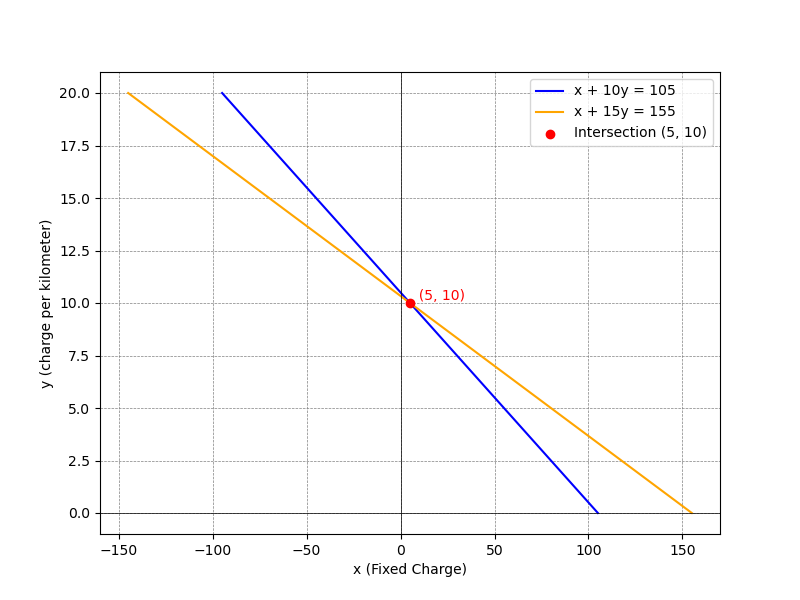
\includegraphics[width=\columnwidth]{figs/Figure_1.png}
		\caption{Solution of the system of linear equations}
		\label{stemplot}
	\end{figure}
\end{document}
